% Options for packages loaded elsewhere
\PassOptionsToPackage{unicode}{hyperref}
\PassOptionsToPackage{hyphens}{url}
\PassOptionsToPackage{dvipsnames,svgnames,x11names}{xcolor}
%
\documentclass[
  11pt,
]{article}
\usepackage{amsmath,amssymb}
\usepackage{lmodern}
\usepackage{iftex}
\ifPDFTeX
  \usepackage[T1]{fontenc}
  \usepackage[utf8]{inputenc}
  \usepackage{textcomp} % provide euro and other symbols
\else % if luatex or xetex
  \usepackage{unicode-math}
  \defaultfontfeatures{Scale=MatchLowercase}
  \defaultfontfeatures[\rmfamily]{Ligatures=TeX,Scale=1}
  \setmainfont[]{Palatino}
\fi
% Use upquote if available, for straight quotes in verbatim environments
\IfFileExists{upquote.sty}{\usepackage{upquote}}{}
\IfFileExists{microtype.sty}{% use microtype if available
  \usepackage[]{microtype}
  \UseMicrotypeSet[protrusion]{basicmath} % disable protrusion for tt fonts
}{}
\makeatletter
\@ifundefined{KOMAClassName}{% if non-KOMA class
  \IfFileExists{parskip.sty}{%
    \usepackage{parskip}
  }{% else
    \setlength{\parindent}{0pt}
    \setlength{\parskip}{6pt plus 2pt minus 1pt}}
}{% if KOMA class
  \KOMAoptions{parskip=half}}
\makeatother
\usepackage{xcolor}
\IfFileExists{xurl.sty}{\usepackage{xurl}}{} % add URL line breaks if available
\IfFileExists{bookmark.sty}{\usepackage{bookmark}}{\usepackage{hyperref}}
\hypersetup{
  colorlinks=true,
  linkcolor={teal},
  filecolor={Maroon},
  citecolor={teal},
  urlcolor={teal},
  pdfcreator={LaTeX via pandoc}}
\urlstyle{same} % disable monospaced font for URLs
\usepackage[left=3cm,right=3cm,top=2cm,bottom=2cm]{geometry}
\usepackage{longtable,booktabs,array}
\usepackage{calc} % for calculating minipage widths
% Correct order of tables after \paragraph or \subparagraph
\usepackage{etoolbox}
\makeatletter
\patchcmd\longtable{\par}{\if@noskipsec\mbox{}\fi\par}{}{}
\makeatother
% Allow footnotes in longtable head/foot
\IfFileExists{footnotehyper.sty}{\usepackage{footnotehyper}}{\usepackage{footnote}}
\makesavenoteenv{longtable}
\usepackage{graphicx}
\makeatletter
\def\maxwidth{\ifdim\Gin@nat@width>\linewidth\linewidth\else\Gin@nat@width\fi}
\def\maxheight{\ifdim\Gin@nat@height>\textheight\textheight\else\Gin@nat@height\fi}
\makeatother
% Scale images if necessary, so that they will not overflow the page
% margins by default, and it is still possible to overwrite the defaults
% using explicit options in \includegraphics[width, height, ...]{}
\setkeys{Gin}{width=\maxwidth,height=\maxheight,keepaspectratio}
% Set default figure placement to htbp
\makeatletter
\def\fps@figure{htbp}
\makeatother
\setlength{\emergencystretch}{3em} % prevent overfull lines
\providecommand{\tightlist}{%
  \setlength{\itemsep}{0pt}\setlength{\parskip}{0pt}}
\setcounter{secnumdepth}{-\maxdimen} % remove section numbering
\newlength{\cslhangindent}
\setlength{\cslhangindent}{1.5em}
\newlength{\csllabelwidth}
\setlength{\csllabelwidth}{3em}
\newlength{\cslentryspacingunit} % times entry-spacing
\setlength{\cslentryspacingunit}{\parskip}
\newenvironment{CSLReferences}[2] % #1 hanging-ident, #2 entry spacing
 {% don't indent paragraphs
  \setlength{\parindent}{0pt}
  % turn on hanging indent if param 1 is 1
  \ifodd #1
  \let\oldpar\par
  \def\par{\hangindent=\cslhangindent\oldpar}
  \fi
  % set entry spacing
  \setlength{\parskip}{#2\cslentryspacingunit}
 }%
 {}
\usepackage{calc}
\newcommand{\CSLBlock}[1]{#1\hfill\break}
\newcommand{\CSLLeftMargin}[1]{\parbox[t]{\csllabelwidth}{#1}}
\newcommand{\CSLRightInline}[1]{\parbox[t]{\linewidth - \csllabelwidth}{#1}\break}
\newcommand{\CSLIndent}[1]{\hspace{\cslhangindent}#1}
\usepackage[labelsep=period]{caption}
\usepackage[labelfont=bf]{caption}
\usepackage[switch]{lineno}
\usepackage{type1cm} % scalable fonts
\usepackage{lettrine}
\usepackage{booktabs}
\usepackage{sectsty} \sectionfont{\centering}
\usepackage{caption}
\captionsetup[figure]{font=footnotesize}
\captionsetup[table]{font=footnotesize}
\captionsetup[table]{justification=centerlast}
\captionsetup[figure]{justification=centerlast}
\usepackage{booktabs}
\usepackage{longtable}
\usepackage{array}
\usepackage{multirow}
\usepackage{wrapfig}
\usepackage{float}
\usepackage{colortbl}
\usepackage{pdflscape}
\usepackage{tabu}
\usepackage{threeparttable}
\usepackage{threeparttablex}
\usepackage[normalem]{ulem}
\usepackage{makecell}
\usepackage{xcolor}
\ifLuaTeX
  \usepackage{selnolig}  % disable illegal ligatures
\fi

\author{}
\date{\vspace{-2.5em}}

\begin{document}

\captionsetup{justification=raggedright,singlelinecheck=false}
\pagenumbering{gobble}

%\begin{titlepage}
\begin{center}
\begin{figure}[h!]
\centering
  
\includegraphics[width=10cm]{../images/uoy_logo.png}
  \label{}
\end{figure}
\vspace*{2\baselineskip}
\Large{\textbf{Working Title}}\\
Natasha Hopkins\\
\vspace*{2\baselineskip}
\Large{\textbf{82H Project for Master of Biology (MBiol)}}\\
\Large{Univeristy of York, UK}\\
\vspace*{2\baselineskip}
\Large{\textbf{Project Director}}\\
Dr. Richard Maguire\\
\vspace*{2\baselineskip}
\Large{\textbf{Examination Date}}\\
18 April, 2022
\end{center}

% \end{titlepage}
\hypersetup{linkcolor = black}
\newpage
\tableofcontents
\hypersetup{linkcolor = teal}

\newpage
\linenumbers
\pagenumbering{arabic}
\rule{\textwidth}{0.4pt}\\
\lettrine[lines=2,slope=0pt,nindent=0pt, loversize=0.2]{S}{hear} stress alters endothelial responses via developmental pathways. This is thought to play a role in atherosclerosis formation in regions of low shear stress. One feature of atherosclerosis is an increase in angiogenesis. \\

\begin{center}
\textbf{\textit{Key Words:}} Atherosclerosis • Wnt/βeta-catenin Signalling Pathway • Shear Stress • Orbital Shaker • Angiopoietin-2 • Thrombospondin-1\\
\end{center}

\begin{flushright}
(250 Words)\\
\end{flushright}
\rule{\textwidth}{0.4pt}

\hypertarget{introduction}{%
\section{Introduction}\label{introduction}}

Atherosclerosis is a chronic inflammatory disease characterised by the formation of arterial plaques.
Haemodynamic shear stress has been identified as a modulator of site-specificity in atherosclerosis, which occurs preferentially in regions exposed to low, oscillatory shear stress (\protect\hyperlink{ref-stone2007}{Stone et al., 2007}). Whereas areas of high, laminar shear stress are atheroprotective (\protect\hyperlink{ref-timmins2017}{Timmins et al., 2017}). Shear stress is an important factor in regulating gene expression in vascular endothelial cells (\protect\hyperlink{ref-Ni2010}{Ni et al., 2010}), which is thought to contribute to the susceptibility of plaque formation in atheroprone sites. Multiple omics studies have implicated variations in flow with the regulation of developmental signalling pathways in atherosclerosis, including the Wnt Pathway (\protect\hyperlink{ref-Souilhol2020}{Souilhol et al., 2019}; \protect\hyperlink{ref-Gelfand2011}{Gelfand et al., 2011}).

Wnt is an evolutionarily conserved pathway with a critical role in axis patterning during embryonic development.
In the absence of Wnt, axin forms a destruction complex with glycogen synthase kinase 3β (GSK-3) and adenomatous polyposis coli (APC), which phosphorylates β-catenin and targets it for degradation.
However, in the active canonical Wnt pathway, Wnt ligands interact with Frizzled and LRP receptors.
This leads to the translocation of axin, inhibiting the formation of the destruction complex, allowing β-catenin to accumulate and translocate to the nucleus, where it will activate the transcription of Wnt target genes (\protect\hyperlink{ref-gordon2006}{Gordon and Nusse, 2006}). Of these includes axin, which acts as a negative regulator of Wnt signalling (\protect\hyperlink{ref-Jho2002}{Jho et al., 2002}; \protect\hyperlink{ref-Lustig2002}{Lustig et al., 2002}).

Shear stress-mediated Wnt orchestrates a range of endothelial responses, including angiogenesis, which is increased in regions of low shear stress compared to high shear stress (\protect\hyperlink{ref-du2018}{Du and Li, 2018}). One target of Wnt, angiopoietin-2 (ANGPT2), is an established growth factor involved in angiogenesis. Studies in both zebrafish and mice have shown that the increase in ANGPT2 contributes to the development of atherosclerosis (\protect\hyperlink{ref-Li2014-mx}{Li et al., 2014}; \protect\hyperlink{ref-farhat2013}{Farhat et al., 2013a}).

Thrombospondin-1 (THBS1) is a glycoprotein involved in endothelial cell interactions and is a potential target of Wnt.
High levels of THBS1 has been correlated with the inhibition of tumour angiogenesis (\protect\hyperlink{ref-naumov2006}{Naumov et al., 2006}), possibly by induction of apoptosis via the TGF-β pathway (\protect\hyperlink{ref-Miao2001}{Miao et al., 2001}; \protect\hyperlink{ref-yee2004}{Yee et al., 2004}), or by inhibition of the VEGF pathway (\protect\hyperlink{ref-gupta1999}{Gupta et al., 1999}; \protect\hyperlink{ref-kaur2010}{Kaur et al., 2010}).
Jo et al. (\protect\hyperlink{ref-jo2005}{2005}) demonstrated that activation of the Wnt pathway downregulates THBS1 in colon cancer.
Thus, Wnt may mediate the expression of THBS1 in response to flow.
Since atherosclerosis occurs in regions of increased angiogenesis, we would expect \emph{THSB1} to be downregulated in low shear stress.
This has been confirmed in a study by Moura et al. (\protect\hyperlink{ref-Moura2008}{2008}).

\begin{figure}

{\centering 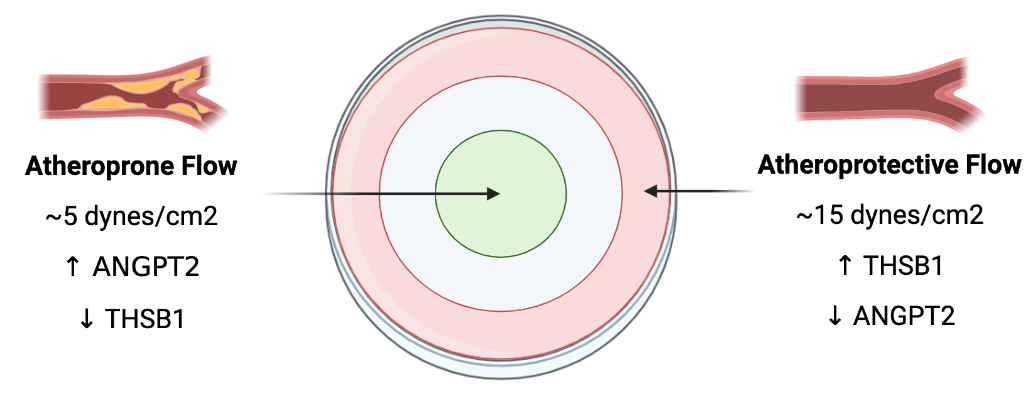
\includegraphics[width=0.8\linewidth]{../images/orbital} 

}

\caption{The orbital shaker model replicates the shear stress exterted in atheroprone and atheroprotective regions. Image created with BioRender.}\label{fig:orbital}
\end{figure}

In our study, we aimed to compare the expression of \emph{ANGPT2} and \emph{THBS1} in HUVECs exposed to atheroprone low shear stress (LSS) and atheroprotective high shear stress (HSS) using an orbital shaker model.
The model, described by Warboys et al. (\protect\hyperlink{ref-Warboys2014}{2014}), exposes cells to variable stress of approximately 5 dynes in the centre and approximately 15 dynes in the periphery of the plate (Figure \ref{fig:orbital}).
The purpose of this is to replicate the forces exerted in atheroprone and atheroprotective regions, respectively.
Based on the prior work mentioned, we expect LSS to upregulate \emph{ANGPT2} and downregulate \emph{THSB1} when compared to HSS.
We also used an inhibitor to examine whether altered expression of these genes is controlled by shear stress mediated canonical Wnt signalling.

\color{red}

\begin{itemize}
\item
  introduce orbital shaker model
\item
  explicitly explain aims
\end{itemize}

\color{black}

\hypertarget{materials-and-methods}{%
\section{Materials and Methods}\label{materials-and-methods}}

\hypertarget{cell-culture-and-application-of-shear-stress}{%
\subsection{Cell Culture and Application of Shear Stress}\label{cell-culture-and-application-of-shear-stress}}

HUVECs were cultured at 37°C in 8\% M199, 0.15\% sodium bicarbonate, 1 U/mL pen-strep, 0.1 ug/ml amphotericin B, 20\% Hi-FBS, 30 ug/ml endothelial cell growth supplement (ECGS), and 10 U/ml heparin.
After reaching \textasciitilde80\% confluence, passage 2 cells were incubated with 1ml of trypsin until cells thoroughly detached, and neutralised with 9ml of M199.
They were then re-suspended in M199 media before transferring to 10mm radius 6 well plates coated in 1\% gelatin.
The canonical Wnt pathway was inhibited using XAV939.
Once confluent, cells were treated with either 3ml of 0.1\% DMSO in M199 or 0.1\% XAV939 in M199 (\protect\hyperlink{ref-Zhu2017}{Zhu et al., 2017}).
They were placed on an orbital shaker at 210 rpm for 72 hours, and exposed to low (\textasciitilde5 dynes/cm\textsuperscript{2}) and high shear stress (\textasciitilde15 dynes/cm\textsuperscript{2}) (\protect\hyperlink{ref-Warboys2019}{Warboys, Ghim and Weinberg, 2019}), with the exception of the static control.

\hypertarget{rna-extraction-and-real-time-quantitative-pcr}{%
\subsection{RNA Extraction and Real-Time Quantitative PCR}\label{rna-extraction-and-real-time-quantitative-pcr}}

Cells were isolated from the periphery and centre of the plates with cold PBS and centrifuged for 5 minutes at 400g.
Total mRNA was extracted using the RNEasy Mini Kit (Qiagen) and the concentration was determined spectrophotometrically.
cDNA synthesis was performed using the Verso cDNA Synthesis Kit (Thermo Scientific) as per the manufacturers instructions.
\emph{ANGPT2}, \emph{AXIN2}, \emph{THSB1}, and \emph{HPRT1} (reference gene) mRNA was quantified using StepOne qPCR (Thermo Scientific) with SYBR Green, using oligonucleotide qPCR primers from Ensembl (\protect\hyperlink{ref-howe2020}{Howe et al., 2020}) (Table \ref{tab:primers}).
The amplification included 30 cycles at 95°C for 30s, 5°C for 30s, and 72°C for 45s, followed by 72 °C 10 min.

\begin{table}[!h]

\caption{\label{tab:primers}Oligonucleotide qPCR primers from Ensembl.}
\begin{tabu} to \linewidth {>{\raggedright}X>{\raggedright}X>{\raggedright\arraybackslash}p{8cm}}
\toprule
Gene & Direction & Sequence\\
\midrule
 & L & CGGCTGTGATGATAGAAATAGGGA\\

\multirow{-2}{*}{\raggedright\arraybackslash ANGPT2} & R & GTTCCAAGAGCTGAAGTTCAAGTC\\

 & L & TGTCACTTACTTTTTCTGTGGGGA\\

\multirow{-2}{*}{\raggedright\arraybackslash AXIN1} & R & TGTCACTTACTTTTTCTGTGGGGA\\

 & L & TTGGTCAGGCAGTATAATCC\\

\multirow{-2}{*}{\raggedright\arraybackslash HPRT1} & R & GGGCATATCCTACAACAAC\\

 & L & AAAGATGGAGAATGCTGAGTTGGA\\

\multirow{-2}{*}{\raggedright\arraybackslash THSB1} & R & GGTTCCAAAGACAAACCTCACATT\\
\bottomrule
\end{tabu}
\end{table}

\hypertarget{statistical-analysis}{%
\subsection{Statistical Analysis}\label{statistical-analysis}}

Relative expression is expressed as 2\textsuperscript{ΔΔCt} fold change ± SEM, normalised to the HPRT control.
Normality was determined with Kolmogorov-Smirnov Tests.
Comparison analysis was performed using the Student's t-test.
All plots and analyses were performed in R (\protect\hyperlink{ref-R}{R Core Team, 2018}).

\hypertarget{results}{%
\section{Results}\label{results}}

To asses the effect of low and high shear stress on gene express, HUVECs were exposed to flow using an orbital shaker system.
Gene expression of \emph{ANGPT2}, \emph{THSB1}, and Wnt reporter \emph{AXIN2} was quantified by qPCR.
Gene expression in HUVECs exposed LSS was compared to those exposed to HSS (Figure \ref{fig:plots}A).
Low shear stress downregulated the expression of \emph{AXIN2}, \emph{ANGPT2}, and \emph{THBS1}.
\emph{AXIN2}, a known Wnt target, decreased by 0.28-fold in low shear stress.
Similarly, \emph{ANGPT2} was decreased by 0.15-fold, and THBS1 was decreased 0.12-fold.
Using the same method, HUVECs were also treated with either DMSO or canonical Wnt inhibitor XAV929, to assess for regulation by Wnt signalling.
Expression in the presence of XAV939 was then compared to DMSO (Figure \ref{fig:plots}B).
Exposure to LSS with the addition XAV939 intensified the expression of \emph{AXIN2} by 18.82-fold, \emph{ANGPT} by 33.35-fold, and \emph{THBS1} by 35.59-fold.
Whereas XAV929 decreased expression in HSS.
\emph{AXIN2} decreased 0.68-fold, \emph{ANGPT2} by 0.42-fold, and \emph{THBS1} by 0.87-fold.
Results were analysed using the Students \emph{t} test, which regarded them insignificant due to the small sample size.

\begin{figure}

{\centering 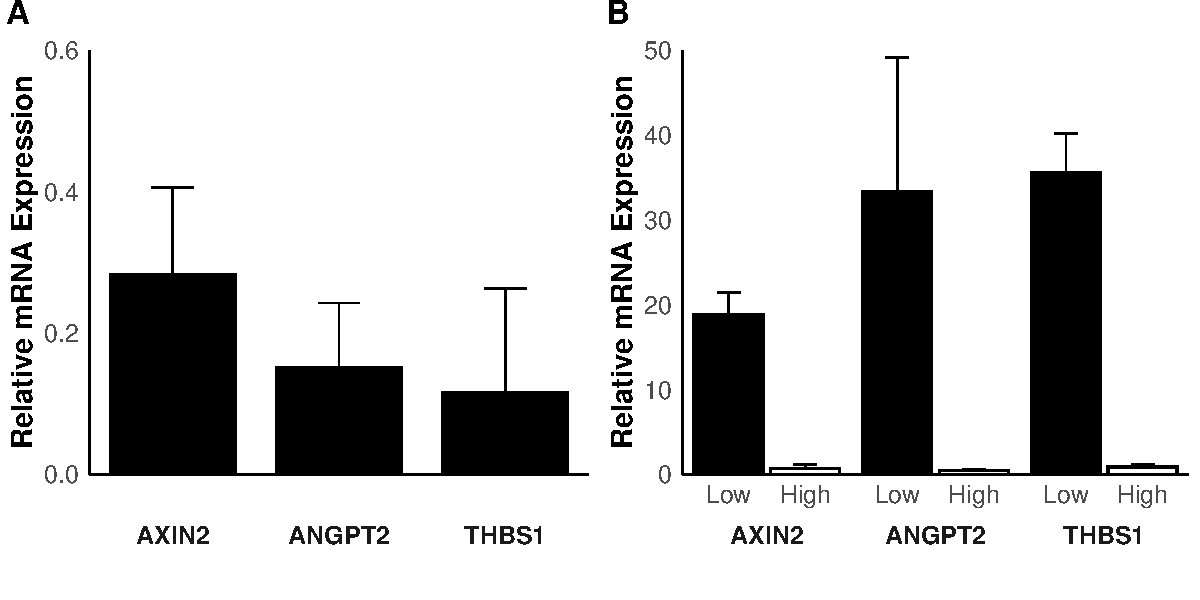
\includegraphics{report_files/figure-latex/plots-1} 

}

\caption{Low shear stress downregulates AXIN2, ANGPT2, and THSB1 expression via Wnt signalling. Cells were treated with DMSO(-) or XAV939(+) and exposed to low or high shear stress. Levels of angiopoietin-2, axin-2, and thrombospondin-1 mRNA were quantified by qPCR. (\textbf{A}) Low shear stress upregulated the expression of all genes. \emph{AXIN}: 0.28±0.12, \emph{ANGPT2}: 0.15±0.09, \emph{THBS1}: 0.12±0.15. Data is shown as fold change ± SEM of low shear stress relative to high shear stress. (\textbf{B}) XAV939 upregulated expression of all genes in low shear stress and downregulated expression of all genes in high shear stress. \emph{AXIN}: 18.82±2.66 and 0.68±0.50. \emph{ANGPT2}: 33.36±15.80 and 0.42±0.14, \emph{THBS1}: 35.59±4.55 and 0.87±0.33. Data is shown as fold change ± SEM of XAV939 relative to DMSO.}\label{fig:plots}
\end{figure}

\hypertarget{discussion}{%
\section{Discussion}\label{discussion}}

In our study, we compare the effects of low shear stress and high shear stress on the expression of two regulators of angiogenesis, \emph{ANGPT2} and \emph{THBS1}, and whether their expression is controlled by Wnt.
This was achieved using an orbital shaker model, first described by Warboys et al. (\protect\hyperlink{ref-Warboys2014}{2014}).
Direct Wnt target, \emph{AXIN2}, was also measured to quantify Wnt expression (\protect\hyperlink{ref-Jho2002}{Jho et al., 2002}).
Finally, we compared gene expression in LSS to HSS, and XAV939 to DMSO.

Our findings indicate that \emph{AXIN2}, \emph{ANGPT}, and \emph{THBS1} is downregulated in HUVECs exposed to LSS (Figure \ref{fig:plots}A).
The downregulation of \emph{ANGPT} and \emph{AXIN2} in LSS differs from our expectations.
Previous studies demonstrate that canonical Wnt is activated by low shear stress (\protect\hyperlink{ref-Gelfand2011}{Gelfand et al., 2011}), as is its direct target, \emph{AXIN2} (\protect\hyperlink{ref-Jho2002}{Jho et al., 2002}).
\emph{ANGPT2}, a positive regulator of angiogenesis, has also been identified as a positive target of Wnt in zebrafish (\protect\hyperlink{ref-Li2014-mx}{Li et al., 2014}).
Thus, \emph{ANGPT2} was also expected to be upregulated in LSS.
However, the results imply that Wnt is downregulated by LSS compared to HSS, and in doing so, downregulates both \emph{ANGPT2} and \emph{AXIN2}.

On the other hand, the lower expression of \emph{THSB1} in low shear stress was anticipated (\protect\hyperlink{ref-Moura2008}{Moura et al., 2008}).
Wnt has been shown to inhibit \emph{THBS1}, a negative regulator of angiogenesis, in colonic tumours (\protect\hyperlink{ref-jo2005}{Jo et al., 2005}).
Therefore, its expression should increase with the downregulation of \emph{AXIN2}.
This was not the case, suggesting that it is not repressed by the Wnt pathway as previously reported.

\color{red}

\begin{itemize}
\tightlist
\item
  This is a very different context - you should make this clear, and if it's the basis of choosing it as a target mention it in the introduction. If it's not regulated by Wnt in this context - then that is fine but you need to be quite explicit in how you discuss it.
\end{itemize}

\color{black}

In the presence of XAV939, all genes were upregulated in both low and high shear stress (Figure \ref{fig:plots}B).
Initially, this would imply that Wnt is an inhibitor of \emph{ANGPT2} and \emph{THSB1}.

However, since \emph{AXIN2} is a direct inhibitor of Wnt, this suggests that the inhibitor in fact failed to inhibit Wnt.
?

\color{red}

\begin{itemize}
\item
  Maybe - how could you find out?
  Also - is this canonical or non-canonical Wnt?
  There is cross talk between the two kinds of pathway, but they are quite separate.
  XAV939 won't inhibit non-canonical Wnt signalling.

  \begin{itemize}
  \tightlist
  \item
    These Are where the marks are. You should think about how you could confirm if you are inhibiting signalling (usually a WEstern blot for phospho proteins involved in the signalling pathway - if you look up the vendor page of the inhibition there is usually a paper where they confirm the inhibitor in some system or another).
  \end{itemize}
\item
  If Inhibitor failed, why not consistent with the DMSO samples?

  \begin{itemize}
  \tightlist
  \item
    XAV939 works but issue with primers specificity? Bind to another protein upregulated in LSS. Wnt downregulated in HSS hence why fold changes smaller? Small sample size so downregulation seems more prominent then it actually is
  \end{itemize}
\end{itemize}

\color{black}

There are many discrepancies between our results and prior studies, likely due to limitations and errors in our method\ldots{}

\color{red}

\begin{itemize}
\item
  Possible Errors and Refine Methods

  \begin{itemize}
  \item
    Small sample = not enough to confirm spectrophotometer was consistent
  \item
    No prior PCR experience
  \end{itemize}
\item
  Melt curve suggests primer dimers and contamination (include images of curves or include in supplementary?)
\item
  en face staining for gene markers in inner curvature (\protect\hyperlink{ref-Warboys2014}{Warboys et al., 2014})
\item
  Direct interaction with Wnt or via VEGF?

  \begin{itemize}
  \tightlist
  \item
    \emph{THSB1} inhibits VEGF by competing for heparin (which is used in our medium) (\protect\hyperlink{ref-gupta1999}{Gupta et al., 1999}; \protect\hyperlink{ref-dias2012}{Dias et al., 2012}; \protect\hyperlink{ref-tolsma1993}{Tolsma et al., 1993})
  \end{itemize}
\item
  Then you can start tying in non canonical Wnt signalling and seeing whether there is cross talk with either this pathway or other pathways that could explain the result.
  Then what sort of experiments in other systems you could do.
\item
  Methods used in other studies
\item
  animal studies, zebrafish, mice, pigs {[}Serbanovic-Canic et al. (\protect\hyperlink{ref-serbanovic-canic2017}{2017}); Li et al. (\protect\hyperlink{ref-Li2014-mx}{2014}); Farhat et al. (\protect\hyperlink{ref-farhat2013a}{2013b}); Moura et al. (\protect\hyperlink{ref-Moura2008}{2008}); Moonen et al. (\protect\hyperlink{ref-moonen2015}{2015})
\item
  non-canonical wnt (\protect\hyperlink{ref-franco2016}{Franco et al., 2016})
\item
  relative vs quantitative expression
\item
  flow chamber instead of orbital shaker
\end{itemize}

\color{black}

\hypertarget{acknowledgements}{%
\section{Acknowledgements}\label{acknowledgements}}

\begin{flushright}
Word Count: 1645 Words
\end{flushright}

\hypertarget{references}{%
\section{References}\label{references}}

\small

\hypertarget{refs}{}
\begin{CSLReferences}{0}{0}
\leavevmode\vadjust pre{\hypertarget{ref-dias2012}{}}%
\CSLLeftMargin{1. }
\CSLRightInline{Dias, J. V. {et al.} (2012). {A motif within the N-terminal domain of TSP-1 specifically promotes the proangiogenic activity of endothelial colony-forming cells}. \emph{Biochemical Pharmacology}, 84 (8), pp.1014--1023. {[}Online{]}. Available at: doi:\href{https://doi.org/10.1016/j.bcp.2012.07.006}{10.1016/j.bcp.2012.07.006}.}

\leavevmode\vadjust pre{\hypertarget{ref-du2018}{}}%
\CSLLeftMargin{2. }
\CSLRightInline{Du, J. and Li, J. (2018). {The role of wnt signaling pathway in atherosclerosis and its relationship with angiogenesis}. \emph{Experimental and Therapeutic Medicine}. {[}Online{]}. Available at: doi:\href{https://doi.org/10.3892/etm.2018.6397}{10.3892/etm.2018.6397}.}

\leavevmode\vadjust pre{\hypertarget{ref-farhat2013}{}}%
\CSLLeftMargin{3. }
\CSLRightInline{Farhat, N. {et al.} (2013a). {Angiopoietin{-}Like 2 Promotes Atherogenesis in Mice}. \emph{Journal of the American Heart Association}, 2 (3). {[}Online{]}. Available at: doi:\href{https://doi.org/10.1161/jaha.113.000201}{10.1161/jaha.113.000201}.}

\leavevmode\vadjust pre{\hypertarget{ref-farhat2013a}{}}%
\CSLLeftMargin{4. }
\CSLRightInline{Farhat, N. {et al.} (2013b). {Angiopoietin{-}Like 2 Promotes Atherogenesis in Mice}. \emph{Journal of the American Heart Association}, 2 (3). {[}Online{]}. Available at: doi:\href{https://doi.org/10.1161/jaha.113.000201}{10.1161/jaha.113.000201}.}

\leavevmode\vadjust pre{\hypertarget{ref-franco2016}{}}%
\CSLLeftMargin{5. }
\CSLRightInline{Franco, C. A. {et al.} (2016). {Non-canonical Wnt signalling modulates the endothelial shear stress flow sensor in vascular remodelling}. \emph{eLife}, 5. {[}Online{]}. Available at: doi:\href{https://doi.org/10.7554/elife.07727}{10.7554/elife.07727}.}

\leavevmode\vadjust pre{\hypertarget{ref-Gelfand2011}{}}%
\CSLLeftMargin{6. }
\CSLRightInline{Gelfand, B. D. {et al.} (2011). {Hemodynamic Activation of β-Catenin and T-Cell-Specific Transcription Factor Signaling in Vascular Endothelium Regulates Fibronectin Expression}. \emph{Arteriosclerosis, Thrombosis, and Vascular Biology}, 31 (7), pp.1625--1633. {[}Online{]}. Available at: doi:\href{https://doi.org/10.1161/atvbaha.111.227827}{10.1161/atvbaha.111.227827}.}

\leavevmode\vadjust pre{\hypertarget{ref-gordon2006}{}}%
\CSLLeftMargin{7. }
\CSLRightInline{Gordon, M. D. and Nusse, R. (2006). {Wnt Signaling: Multiple Pathways, Multiple Receptors, and Multiple Transcription Factors}. \emph{Journal of Biological Chemistry}, 281 (32), pp.22429--22433. {[}Online{]}. Available at: doi:\href{https://doi.org/10.1074/jbc.r600015200}{10.1074/jbc.r600015200}.}

\leavevmode\vadjust pre{\hypertarget{ref-gupta1999}{}}%
\CSLLeftMargin{8. }
\CSLRightInline{Gupta, K. {et al.} (1999). \emph{Angiogenesis}, 3 (2), pp.147--158. {[}Online{]}. Available at: doi:\href{https://doi.org/10.1023/a:1009018702832}{10.1023/a:1009018702832}.}

\leavevmode\vadjust pre{\hypertarget{ref-howe2020}{}}%
\CSLLeftMargin{9. }
\CSLRightInline{Howe, K. L. {et al.} (2020). {Ensembl 2021}. \emph{Nucleic Acids Research}, 49 (D1), pp.D884--D891. {[}Online{]}. Available at: doi:\href{https://doi.org/10.1093/nar/gkaa942}{10.1093/nar/gkaa942}.}

\leavevmode\vadjust pre{\hypertarget{ref-Jho2002}{}}%
\CSLLeftMargin{10. }
\CSLRightInline{Jho, E. {et al.} (2002). {Wnt/β-Catenin/Tcf Signaling Induces the Transcription of Axin2, a Negative Regulator of the Signaling Pathway}. \emph{Molecular and Cellular Biology}, 22 (4), pp.1172--1183. {[}Online{]}. Available at: doi:\href{https://doi.org/10.1128/mcb.22.4.1172-1183.2002}{10.1128/mcb.22.4.1172-1183.2002}.}

\leavevmode\vadjust pre{\hypertarget{ref-jo2005}{}}%
\CSLLeftMargin{11. }
\CSLRightInline{Jo, W.-S. {et al.} (2005). {Wnt signaling can repress thrombospondin-1 expression in colonic tumorigenesis}. \emph{Cancer Biology \& Therapy}, 4 (12), pp.1361--1366. {[}Online{]}. Available at: doi:\href{https://doi.org/10.4161/cbt.4.12.2201}{10.4161/cbt.4.12.2201}.}

\leavevmode\vadjust pre{\hypertarget{ref-kaur2010}{}}%
\CSLLeftMargin{12. }
\CSLRightInline{Kaur, S. {et al.} (2010). {Thrombospondin-1 Inhibits VEGF Receptor-2 Signaling by Disrupting Its Association with CD47}. \emph{Journal of Biological Chemistry}, 285 (50), pp.38923--38932. {[}Online{]}. Available at: doi:\href{https://doi.org/10.1074/jbc.m110.172304}{10.1074/jbc.m110.172304}.}

\leavevmode\vadjust pre{\hypertarget{ref-Li2014-mx}{}}%
\CSLLeftMargin{13. }
\CSLRightInline{Li, R. {et al.} (2014). {Shear stress-activated wnt-angiopoietin-2 signaling recapitulates vascular repair in zebrafish embryos}. \emph{Arteriosclerosis, thrombosis, and vascular biology}, 34 (10), pp.2268--2275.}

\leavevmode\vadjust pre{\hypertarget{ref-Lustig2002}{}}%
\CSLLeftMargin{14. }
\CSLRightInline{Lustig, B. {et al.} (2002). {Negative Feedback Loop of Wnt Signaling through Upregulation of Conductin/Axin2 in Colorectal and Liver Tumors}. \emph{Molecular and Cellular Biology}, 22 (4), pp.1184--1193. {[}Online{]}. Available at: doi:\href{https://doi.org/10.1128/mcb.22.4.1184-1193.2002}{10.1128/mcb.22.4.1184-1193.2002}.}

\leavevmode\vadjust pre{\hypertarget{ref-Miao2001}{}}%
\CSLLeftMargin{15. }
\CSLRightInline{Miao, W. M. {et al.} (2001). {Thrombospondin-1 type 1 repeat recombinant proteins inhibit tumor growth through transforming growth factor-beta-dependent and -independent mechanisms.} \emph{Cancer research}, 61 21, pp.7830--7839.}

\leavevmode\vadjust pre{\hypertarget{ref-moonen2015}{}}%
\CSLLeftMargin{16. }
\CSLRightInline{Moonen, J.-R. A. J. {et al.} (2015). {Endothelial-to-mesenchymal transition contributes to fibro-proliferative vascular disease and is modulated by fluid shear stress}. \emph{Cardiovascular Research}, 108 (3), pp.377--386. {[}Online{]}. Available at: doi:\href{https://doi.org/10.1093/cvr/cvv175}{10.1093/cvr/cvv175}.}

\leavevmode\vadjust pre{\hypertarget{ref-Moura2008}{}}%
\CSLLeftMargin{17. }
\CSLRightInline{Moura, R. {et al.} (2008). {Thrombospondin-1 Deficiency Accelerates Atherosclerotic Plaque Maturation in {\emph{ApoE}} {\textsuperscript{{-}/{-}}} Mice}. \emph{Circulation Research}, 103 (10), pp.1181--1189. {[}Online{]}. Available at: doi:\href{https://doi.org/10.1161/circresaha.108.185645}{10.1161/circresaha.108.185645}.}

\leavevmode\vadjust pre{\hypertarget{ref-naumov2006}{}}%
\CSLLeftMargin{18. }
\CSLRightInline{Naumov, G. N. {et al.} (2006). {A Model of Human Tumor Dormancy: An Angiogenic Switch From the Nonangiogenic Phenotype}. \emph{JNCI: Journal of the National Cancer Institute}, 98 (5), pp.316--325. {[}Online{]}. Available at: doi:\href{https://doi.org/10.1093/jnci/djj068}{10.1093/jnci/djj068}.}

\leavevmode\vadjust pre{\hypertarget{ref-Ni2010}{}}%
\CSLLeftMargin{19. }
\CSLRightInline{Ni, C.-W. {et al.} (2010). {Discovery of novel mechanosensitive genes in vivo using mouse carotid artery endothelium exposed to disturbed flow}. \emph{Blood}, 116 (15), pp.e66--e73. {[}Online{]}. Available at: doi:\href{https://doi.org/10.1182/blood-2010-04-278192}{10.1182/blood-2010-04-278192}.}

\leavevmode\vadjust pre{\hypertarget{ref-R}{}}%
\CSLLeftMargin{20. }
\CSLRightInline{R Core Team. (2018). {\emph{R: A language and environment for statistical computing}}. Vienna, Austria: R Foundation for Statistical Computing. {[}Online{]}. Available at: \url{https://www.R-project.org/}.}

\leavevmode\vadjust pre{\hypertarget{ref-serbanovic-canic2017}{}}%
\CSLLeftMargin{21. }
\CSLRightInline{Serbanovic-Canic, J. {et al.} (2017). {Zebrafish Model for Functional Screening of Flow-Responsive Genes}. \emph{Arteriosclerosis, Thrombosis, and Vascular Biology}, 37 (1), pp.130--143. {[}Online{]}. Available at: doi:\href{https://doi.org/10.1161/atvbaha.116.308502}{10.1161/atvbaha.116.308502}.}

\leavevmode\vadjust pre{\hypertarget{ref-Souilhol2020}{}}%
\CSLLeftMargin{22. }
\CSLRightInline{Souilhol, C. {et al.} (2019). {Endothelial responses to shear stress in atherosclerosis: a novel role for developmental genes}. \emph{Nature Reviews Cardiology}, 17 (1), pp.52--63. {[}Online{]}. Available at: doi:\href{https://doi.org/10.1038/s41569-019-0239-5}{10.1038/s41569-019-0239-5}.}

\leavevmode\vadjust pre{\hypertarget{ref-stone2007}{}}%
\CSLLeftMargin{23. }
\CSLRightInline{Stone, P. H. {et al.} (2007). {Regions of low endothelial shear stress are the sites where coronary plaque progresses and vascular remodelling occurs in humans: an in vivo serial study}. \emph{European Heart Journal}, 28 (6), pp.705--710. {[}Online{]}. Available at: doi:\href{https://doi.org/10.1093/eurheartj/ehl575}{10.1093/eurheartj/ehl575}.}

\leavevmode\vadjust pre{\hypertarget{ref-timmins2017}{}}%
\CSLLeftMargin{24. }
\CSLRightInline{Timmins, L. H. {et al.} (2017). {Oscillatory wall shear stress is a dominant flow characteristic affecting lesion progression patterns and plaque vulnerability in patients with coronary artery disease}. \emph{Journal of The Royal Society Interface}, 14 (127), p.20160972. {[}Online{]}. Available at: doi:\href{https://doi.org/10.1098/rsif.2016.0972}{10.1098/rsif.2016.0972}.}

\leavevmode\vadjust pre{\hypertarget{ref-tolsma1993}{}}%
\CSLLeftMargin{25. }
\CSLRightInline{Tolsma, S. {et al.} (1993). {Peptides derived from two separate domains of the matrix protein thrombospondin-1 have anti-angiogenic activity}. \emph{Journal of Cell Biology}, 122 (2), pp.497--511. {[}Online{]}. Available at: doi:\href{https://doi.org/10.1083/jcb.122.2.497}{10.1083/jcb.122.2.497}.}

\leavevmode\vadjust pre{\hypertarget{ref-Warboys2014}{}}%
\CSLLeftMargin{26. }
\CSLRightInline{Warboys, C. M. {et al.} (2014). {Disturbed Flow Promotes Endothelial Senescence via a p53-Dependent Pathway}. \emph{Arteriosclerosis, Thrombosis, and Vascular Biology}, 34 (5), pp.985--995. {[}Online{]}. Available at: doi:\href{https://doi.org/10.1161/atvbaha.114.303415}{10.1161/atvbaha.114.303415}.}

\leavevmode\vadjust pre{\hypertarget{ref-Warboys2019}{}}%
\CSLLeftMargin{27. }
\CSLRightInline{Warboys, C. M., Ghim, M. and Weinberg, P. D. (2019). {Understanding mechanobiology in cultured endothelium: A review of the orbital shaker method}. \emph{Atherosclerosis}, 285, pp.170--177. {[}Online{]}. Available at: doi:\href{https://doi.org/10.1016/j.atherosclerosis.2019.04.210}{10.1016/j.atherosclerosis.2019.04.210}.}

\leavevmode\vadjust pre{\hypertarget{ref-yee2004}{}}%
\CSLLeftMargin{28. }
\CSLRightInline{Yee, K. O. {et al.} (2004). {Expression of the Type-1 Repeats of Thrombospondin-1 Inhibits Tumor Growth Through Activation of Transforming Growth Factor-β}. \emph{The American Journal of Pathology}, 165 (2), pp.541--552. {[}Online{]}. Available at: doi:\href{https://doi.org/10.1016/s0002-9440(10)63319-6}{10.1016/s0002-9440(10)63319-6}.}

\leavevmode\vadjust pre{\hypertarget{ref-Zhu2017}{}}%
\CSLLeftMargin{29. }
\CSLRightInline{Zhu, J. {et al.} (2017). {Regulation of angiogenic behaviors by oxytocin receptor through Gli1-indcued transcription of HIF-1? in human umbilical vein endothelial cells}. \emph{Biomedicine \& Pharmacotherapy}, 90, pp.928--934. {[}Online{]}. Available at: doi:\href{https://doi.org/10.1016/j.biopha.2017.04.021}{10.1016/j.biopha.2017.04.021}.}

\end{CSLReferences}

\end{document}
